\documentclass[11pt]{article}

\usepackage[utf8]{inputenc}
\usepackage[T1]{fontenc}
\usepackage{lmodern}
\usepackage{microtype}
\usepackage[margin=1in]{geometry}
\usepackage{amsmath,amssymb,amsthm}
\usepackage{stmaryrd}
\usepackage{mathpartir}
\usepackage{enumitem}
\usepackage{booktabs}
\usepackage{array}
\usepackage{caption}
\usepackage{forest}
\usepackage{tikz}
\usetikzlibrary{automata, positioning, arrows.meta, calc, fit, shapes.geometric, shapes.multipart, matrix, decorations.pathreplacing}
\usepackage{listings}
\usepackage[hidelinks]{hyperref}

\setlength{\parskip}{4pt}
\captionsetup{font=small, labelfont=bf}

\tikzset{
  >={Stealth[length=2mm]},
  every state/.style={draw, minimum size=7mm, inner sep=1pt, font=\small},
  initial text={},
  caja/.style={draw, minimum width=9mm, minimum height=6mm, font=\small\ttfamily},
  flecha/.style={->, thick},
  nodoarbol/.style={draw, circle, minimum size=6mm, inner sep=1pt, font=\small\ttfamily},
}
\forestset{
  arbol/.style={for tree={font=\small\ttfamily, s sep=3mm, l sep=4mm, align=center}},
}

\lstset{
  basicstyle=\ttfamily\small,
  keywordstyle=\bfseries,
  commentstyle=\itshape,
  columns=fullflexible,
  keepspaces=true,
  frame=lines,
  framerule=0.3pt,
  showstringspaces=false,
  breaklines=true,
  xleftmargin=1em,
  xrightmargin=1em,
  captionpos=b,
  upquote=true,
  literate={¬}{{$\neg$}}1 {λ}{{$\lambda$}}1 {→}{{$\to$}}1 {∨}{{$\vee$}}1
    {∧}{{$\wedge$}}1 {⇒}{{$\Rightarrow$}}1 {♭}{{$\flat$}}1 {♯}{{$\sharp$}}1
    {≤}{{$\le$}}1 {≥}{{$\ge$}}1 {⊢}{{$\vdash$}}1 {α}{{$\alpha$}}1 {β}{{$\beta$}}1
    {γ}{{$\gamma$}}1 {∪}{{$\cup$}}1 {Σ}{{$\Sigma$}}1 {∈}{{$\in$}}1
    {σ}{{$\sigma$}}1 {δ}{{$\delta$}}1 {μ}{{$\mu$}}1 {ν}{{$\nu$}}1 {↦}{{$\mapsto$}}1 {Δ}{{$\Delta$}}1 {Γ}{{$\Gamma$}}1 {τ}{{$\tau$}}1 {ρ}{{$\rho$}}1,
}

\lstdefinelanguage{Rascal}{
  morekeywords={module, import, extend, syntax, lexical, layout, keyword, start,
    data, alias, if, else, for, while, do, return, switch, case, default, visit,
    insert, fail, test, bool, int, str, real, num, list, set, map, rel, tuple,
    node, value, void, true, false, when, throw, try, catch, public, private,
    bottom-up, top-down, innermost, outermost, solve, append, loc, left, right,
    assoc, non-assoc},
  sensitive=true,
  morecomment=[l]{//},
  morecomment=[s]{/*}{*/},
  morestring=[b]",
  alsoletter={-},
}

\lstdefinelanguage{Scheme}{
  morekeywords={define, lambda, let, let*, letrec, if, cond, else, case, and,
    or, begin, set!, quote, delay, force, delay-force, make-promise,
    define-syntax, syntax-rules, define-record-type},
  sensitive=true,
  morecomment=[l]{;},
  morestring=[b]",
  alsoletter={-,!,?,*},
}

\lstdefinelanguage{Swift}{
  morekeywords={func, let, var, if, else, guard, return, print, nil, struct,
    class, protocol, precondition, true, false},
  sensitive=true,
  morecomment=[l]{//},
  morestring=[b]",
}

\lstdefinelanguage{JavaScript}{
  morekeywords={let, const, var, if, else, function, return, for, while, true, false},
  sensitive=true,
  morecomment=[l]{//},
  morestring=[b]",
  morestring=[b]`,
}

\lstdefinelanguage{CommonLisp}{
  morekeywords={defvar, defparameter, defun, defmacro, let, let*, lambda, if,
    cond, progn, setf, quote, function, funcall, eval},
  sensitive=false,
  morecomment=[l]{;},
  morestring=[b]",
  alsoletter={-,*},
}

\newcommand{\codefile}[2]{\lstinputlisting[language=#1]{code/#2}}
\newcommand{\codelines}[4]{\lstinputlisting[language=#1, firstline=#3, lastline=#4]{code/#2}}





\newcommand{\reduces}{\rightarrow}
\newcommand{\Reduces}{\Downarrow}
\newcommand{\step}[3]{\langle #1,\, #2 \rangle \reduces \langle #3}
\newcommand{\steppair}[4]{\langle #1,\, #2 \rangle \reduces \langle #3,\, #4 \rangle}
\newcommand{\bigstep}[3]{\langle #1,\, #2 \rangle \Reduces #3}


\newcommand{\deref}[1]{!#1}
\newcommand{\assign}[2]{#1 := #2}
\newcommand{\seq}[2]{#1 \,;\, #2}
\newcommand{\ift}[3]{\mathbf{if}\ #1\ \mathbf{then}\ #2\ \mathbf{else}\ #3}
\newcommand{\whiledo}[2]{\mathbf{while}\ #1\ \mathbf{do}\ #2}
\newcommand{\fordoo}[4]{\mathbf{for}\ (#1;\ #2;\ #3)\ \{#4\}}


\newcommand{\nil}{\mathbf{nil}}
\newcommand{\cons}[2]{\mathbf{cons}(#1,#2)}
\newcommand{\concat}[2]{\mathbf{concat}(#1,#2)}
\newcommand{\append}[2]{\mathbf{append}(#1,#2)}
\newcommand{\tref}[1]{\mathbf{ref}\ #1}


\newcommand{\unit}{\mathbf{unit}}
\newcommand{\tyint}{\mathbf{int}}
\newcommand{\tybool}{\mathbf{bool}}

% Entornos de teoremas compartidos. Los nombres van en inglés porque las
% notas están en inglés.
\theoremstyle{definition}
\newtheorem{definition}{Definition}[section]
\newtheorem{example}[definition]{Example}
\newtheorem{exercise}[definition]{Exercise}

\theoremstyle{plain}
\newtheorem{theorem}[definition]{Theorem}
\newtheorem{lemma}[definition]{Lemma}
\newtheorem{proposition}[definition]{Proposition}

\theoremstyle{remark}
\newtheorem{remark}[definition]{Remark}


\title{Type Systems}
\author{CG}
\date{\today}

\begin{document}
\maketitle
\tableofcontents

\section{Types}
\label{sec:types}

\begin{definition}
A \textbf{type} is a specification of the operations, the data structure, the
external interface and the internal representation of the elements of a
program, its values.
\end{definition}

A type system gives a programming language a logic: rules that describe which
transformations are allowed on which data. This block follows
Watt~\cite[Ch.~2, 8]{watt2004concepts}, Friedman and
Wand~\cite[Ch.~4]{friedman2008essentials} and
Lee~\cite[Sec.~1.5]{lee2017foundations}.

\subsection{Kinds of typing}

The lecture compares three ways in which languages handle types
(Table~\ref{tab:typing-kinds}).

\begin{table}[h]
\centering
\small
\begin{tabular}{l p{0.3\textwidth} p{0.38\textwidth}}
  \toprule
  Typing & Values & When operations are checked \\
  \midrule
  Strong   & each value has one type & statically, while the program is built \\
  Inferred & each value has one type & statically, from types given by the programmer or deduced from the use of each value \\
  Dynamic  & a value can have different types at different times; at run time it is stored as a pair (value, type tag) & at run time \\
  \bottomrule
\end{tabular}
\caption{Kinds of typing.}
\label{tab:typing-kinds}
\end{table}

Discussions about type systems usually turn around four questions, and a
language answers each one independently:
\begin{itemize}
  \item static or dynamic: are types checked before the program runs or
    while it runs?
  \item strong or weak: may the language reinterpret a value as another type
    without an explicit conversion? In Python \lstinline|"3" + 3| is an
    error; in JavaScript it gives \lstinline|"33"|.
  \item explicit or inferred: does the programmer write the types, or does
    the compiler deduce them?
  \item nominal or structural: are two types compatible because of their
    names, or because of their shape?
\end{itemize}

\subsection{Basic, primitive and composite types}

Following Martin-L\"of, three types are the basis of all others. The empty
type $\bot$ has no elements; it is used to express negation, $\neg A ::= A \to
\bot$. The unit type has a single element, written \texttt{()}, \texttt{unit} or
\texttt{null} depending on the language. The two type has two values,
\texttt{true} and \texttt{false}. All other types have infinitely many elements.

Languages provide \textbf{primitive types} (integers, booleans, characters,
pointers) and let the programmer define \textbf{composite types} (functions,
lists, objects, arrays). Primitive types are defined by the range of values
they represent: \texttt{int} is $-2147483648..2147483647$ and \texttt{byte} is
$-128..127$ in Java, and Ada lets the programmer declare new ranges:
\begin{lstlisting}
type Population is range 0..1e10
type Row is range a..n
\end{lstlisting}
Composite types are built from simpler types by product, sum, mapping or
recursion. The lecture's examples are an Ada record, which is a product of
its fields, and a class hierarchy, which behaves as a disjoint union of the
classes that extend the base class:
\begin{lstlisting}
type Month is (jan, feb, ..., dec)
type Day is range 1..31
type Date is record
  m: Month;
  d: Day;
end record;
\end{lstlisting}

\subsection{Type constructors}

Table~\ref{tab:constructors} lists the constructors of the lecture. The names
$\Sigma$ and $\Pi$ come from Martin-L\"of's type theory, where they generalize
the cartesian product and the function space.

\begin{table}[h]
\centering
\small
\renewcommand{\arraystretch}{1.25}
\begin{tabular}{l l p{0.48\textwidth}}
  \toprule
  Constructor & Notation & Meaning \\
  \midrule
  Function   & $T_1 \to T_2$ & functions from $T_1$ to $T_2$ \\
  $\Sigma$-type & $\sum_{i=1}^{n} T_i = \{(v_1, \dots, v_n) \mid v_i : T_i\}$ & tuples of values of the given types; structures and records \\
  $\Pi$-type & $\prod_{v : T_1} T_2$ & functions whose result type may depend on the input value \\
  Equality   & $\mathit{exp}_1 : T = \mathit{exp}_2 : T$ & the type of proofs that two expressions reduce to the same one, as $2 + 2 = 2 * 2$ \\
  Inductive  & $0 : \mathbb{N}$,\ \ $s : \mathbb{N} \to \mathbb{N}$ & self-referential types built from constants and constructor functions \\
  \bottomrule
\end{tabular}
\caption{Type constructors.}
\label{tab:constructors}
\end{table}

\paragraph{Function types and currying.} The type of a function goes from the
types of its parameters to the type of its result. A function of several
parameters can always be seen as a function of one parameter that returns a
function: a function of two integers that returns an integer has type
$\mathit{int} \times \mathit{int} \to \mathit{int}$, or, curried,
$\mathit{int} \to (\mathit{int} \to \mathit{int})$. This is the currying property,
and the arrow associates to the right, so the parentheses are usually omitted:
$\mathit{int} \to \mathit{int} \to \mathit{int}$.

\paragraph{$\Sigma$ and $\Pi$.} A $\Sigma$-type is the type of tuples: if $T_1,
\dots, T_n$ are types, $\sum T_i$ contains the tuples $(v_1, \dots, v_n)$ with
$v_i : T_i$. A $\Pi$-type is the type of functions, where the type of the output
can depend on the input value: for each element $v$ of $T_1$ the function
returns an element of $T_2$, and $T_2$ may mention $v$. When $T_2$ does not
depend on $v$, $\prod_{v : T_1} T_2$ is just $T_1 \to T_2$. (In programming
languages the word ``sum type'' usually means a disjoint union, as
\texttt{Either} in Haskell; in type theory the disjoint union is written
$A + B$, and $\Sigma$ is a generalized product.)

\paragraph{Inductive types.} An inductive type is defined by constant elements
and constructor functions. The natural numbers of Peano have the constant
$0 : \mathbb{N}$ and the successor $s : \mathbb{N} \to \mathbb{N}$, and the
elements of the type are $0, s0, ss0, sss0, \dots$. Lists and trees are
inductive types too; Section~\ref{sec:recursive} returns to them.

\subsection{Static and dynamic type checking}

\paragraph{Static typing.} Every entity of the program has a type at compile
time, and the type checker verifies that the types are consistent before the
program runs. Its advantages: it catches errors early, it gives guarantees
about the programs, and the hardware can sometimes use the types directly
(an integer known at compile time needs no tag). Its cost: the programmer has
to write the types of the values, which type inference
(Section~\ref{sec:inference}) reduces.

\paragraph{Dynamic typing.} The same checks are made while the program runs.
For that, every value carries its type, as a pair (value, type). The lecture
uses Prolog to show it. A predicate
\texttt{list\_length([\_ | L], N)} computes the length of a list; called with a
list it gives $N = 4$, and called as \texttt{list\_length(9, N)} the tags say
that an \texttt{Int} is not a \texttt{List}, and the error is found only when
the call runs. The same idea in Scheme, with explicit tags:
\codelines{Scheme}{scheme/dynamic.scm}{2}{15}
The test calls \texttt{list-length} with a value tagged \texttt{int} and checks
that the error says \texttt{int is-not list}. Dynamic typing is more flexible
when programming, but execution costs more (the checks are repeated every
time an operation runs), the type information takes storage, and the lecture
adds that it promotes careless programming: an error in a branch that the
tests never execute stays hidden. Figure~\ref{fig:static-dynamic} contrasts
when each approach finds the error.

\begin{figure}[h]
\centering
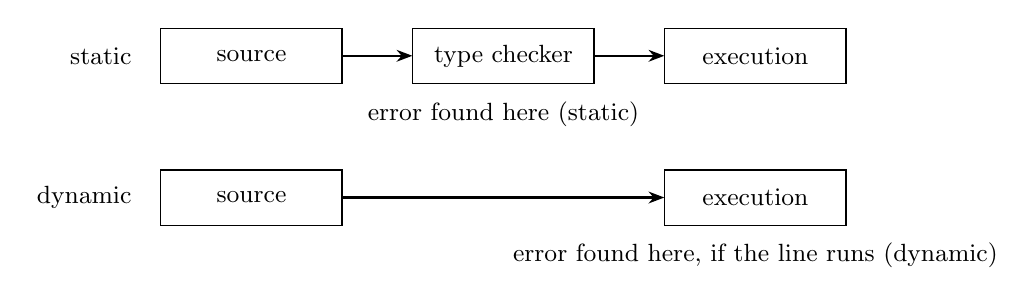
\begin{tikzpicture}[box/.style={draw, minimum width=2.3cm, minimum height=7mm, font=\small}]
  \node[box] (s1) at (0,0) {source};
  \node[box] (s2) at (3.2,0) {type checker};
  \node[box] (s3) at (6.4,0) {execution};
  \draw[flecha] (s1) -- (s2);
  \draw[flecha] (s2) -- (s3);
  \node[font=\small, below=1mm of s2] {error found here (static)};
  \node[box] (d1) at (0,-1.8) {source};
  \node[box] (d3) at (6.4,-1.8) {execution};
  \draw[flecha] (d1) -- (d3);
  \node[font=\small, below=1mm of d3] {error found here, if the line runs (dynamic)};
  \node[font=\small, anchor=east] at (-1.4,0) {static};
  \node[font=\small, anchor=east] at (-1.4,-1.8) {dynamic};
\end{tikzpicture}
\caption{Where a type error is found.}
\label{fig:static-dynamic}
\end{figure}

\paragraph{Duck typing.} Types do not have to be structural: the type of an
expression can also be determined by its behavior. ``If it talks like a duck
and walks like a duck, then it is a duck.'' The lecture shows a Go interface
\texttt{Quacker} that any type with a method \texttt{Quack()} satisfies without
declaring it. In Python the check happens at run time:
\codelines{Python}{python/duck.py}{2}{15}
\texttt{make\_it\_quack} accepts a \texttt{Duck} and a \texttt{Robot}, which have
nothing in common except the method. With a \texttt{Dog} the error appears when
the call runs.

\subsection{Newer types}

Modern type systems add types that make common errors impossible.

\paragraph{Option types.} An option type (or Maybe type) $T?$ holds a value of
$T$ or nothing. It is used for function results that may have no meaningful
value. The lecture writes it in Scala, with \texttt{Some(42)} and
\texttt{None}; in Swift \texttt{Int?} is the same type, with \texttt{nil} for
nothing:
\codelines{Swift}{swift/optionals.swift}{2}{7}
To use the value the program has to open the option (\texttt{if let}), so the
case without a value cannot be forgotten.

\paragraph{Nullable types.} A \texttt{null} value makes operations unsafe: any
expression of a reference type may suddenly be \texttt{null}. A nullable type
system separates $T$ (always a valid reference) from $T?$ (a reference or
\texttt{null}), as in Figure~\ref{fig:nullable}, and the compiler checks that
a $T?$ is never used as a $T$ without a check.
\codelines{Swift}{swift/optionals.swift}{9}{18}
\texttt{greetUser} takes a \texttt{String}, not a \texttt{String?}, so the call
\texttt{greetUser(username: nil)} is rejected at compile time with
\texttt{'nil' is not compatible with expected argument type 'String'}.

\begin{figure}[h]
\centering
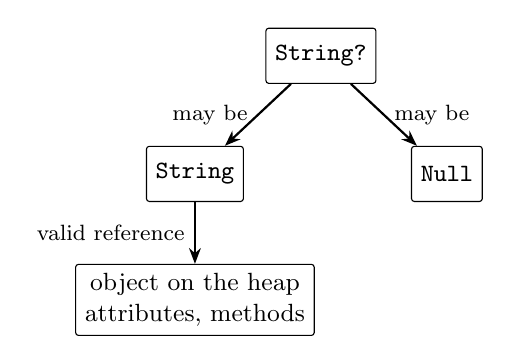
\begin{tikzpicture}[box/.style={draw, rounded corners=1pt, minimum height=7mm, font=\small}]
  \node[box] (opt) at (0,0) {\texttt{String?}};
  \node[box] (str) at (-1.6,-1.5) {\texttt{String}};
  \node[box] (nul) at (1.6,-1.5) {\texttt{Null}};
  \node[box, align=center] (obj) at (-1.6,-3.1) {object on the heap\\attributes, methods};
  \draw[flecha] (opt) -- node[left, font=\footnotesize] {may be} (str);
  \draw[flecha] (opt) -- node[right, font=\footnotesize] {may be} (nul);
  \draw[flecha] (str) -- node[left, font=\footnotesize] {valid reference} (obj);
\end{tikzpicture}
\caption{A nullable type is a valid reference or null.}
\label{fig:nullable}
\end{figure}

\paragraph{Owned types.} In Rust every value is attached to one variable, its
owner, and has exactly one owner at a time. Assigning a value or passing it as
a parameter moves it to a new owner, and the old variable can no longer be
used. A value can also be borrowed (\texttt{\&s}): passed temporarily to a
function and returned to its owner. In the lecture's example,
\texttt{print\_string(s)} moves the string \texttt{s} into the function, so a
second \texttt{print\_string(s)} is a compile error; \texttt{print\_string(\&s)}
only borrows it and can be repeated. Figure~\ref{fig:owned} shows what moves:
the variable holds a pointer, a length and a capacity, and the characters live
on the heap. Moving copies the three fields to the new owner and invalidates
the old one, so the heap memory always has a single owner that frees it.

\begin{figure}[h]
\centering
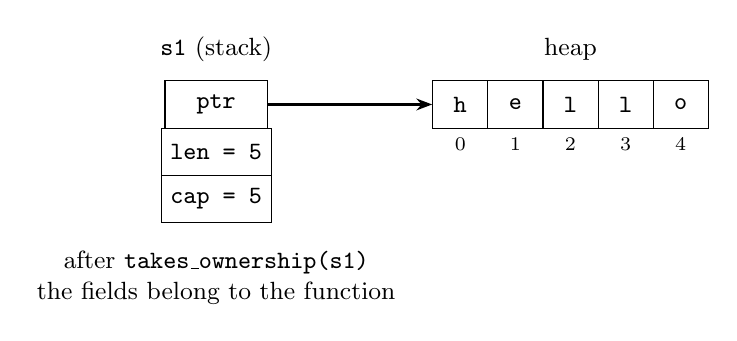
\begin{tikzpicture}[cell/.style={draw, minimum width=1.3cm, minimum height=6mm, font=\small\ttfamily}, hc/.style={draw, minimum width=7mm, minimum height=6mm, font=\small\ttfamily}]
  \node[font=\small] at (0,0.7) {\texttt{s1} (stack)};
  \node[cell] (p) at (0,0) {ptr};
  \node[cell] (l) at (0,-0.6) {len = 5};
  \node[cell] (c) at (0,-1.2) {cap = 5};
  \node[font=\small] at (4.5,0.7) {heap};
  \foreach \ch [count=\i from 0] in {h,e,l,l,o} {
    \node[hc] (h\i) at (3.1+\i*0.7,0) {\ch};
    \node[font=\scriptsize] at (3.1+\i*0.7,-0.5) {\i};
  }
  \draw[flecha] (p.east) -- (h0.west);
  \node[font=\small, align=center] at (0,-2.2) {after \texttt{takes\_ownership(s1)}\\the fields belong to the function};
\end{tikzpicture}
\caption{A Rust \texttt{String}: the owner holds pointer, length and capacity; the text is on the heap.}
\label{fig:owned}
\end{figure}

\subsection{Well-typed programs cannot go wrong}

Robin Milner summarized the goal of static type systems as ``well-typed
programs cannot go wrong''. Going wrong has a precise meaning: reaching a
state where no rule applies, such as applying the number 3 as a function. The
claim is proved as two theorems, progress and preservation, in
Section~\ref{sec:safety}. The sections in between build what the proof needs:
typing rules and the language LETREC (Section~\ref{sec:letrec}), the lambda
calculus and its typed version, type inference, polymorphism, subtyping and
recursive types.

\subsection{Exercises}

\begin{exercise}
Classify Python, Java and Swift by the four questions of this section
(static or dynamic, strong or weak, explicit or inferred, nominal or
structural).
\end{exercise}

\paragraph{Solution.} Python: dynamic, strong, no declarations (types are
checked at run time), and duck typing, which is structural by behavior. Java:
static, strong, explicit (with local inference through \texttt{var}), nominal:
a class is a subtype of an interface only if it declares \texttt{implements}.
Swift: static, strong, inferred where possible, nominal for classes and
protocols (a type conforms to a protocol by declaring it).

\begin{exercise}
Give the type of a curried function \texttt{add} of two integers, and the type
of \texttt{add 3}.
\end{exercise}

\paragraph{Solution.} $\mathit{add} : \mathit{int} \to \mathit{int} \to \mathit{int}$,
which is $\mathit{int} \to (\mathit{int} \to \mathit{int})$. Applying it to 3 gives a
function $\mathit{int} \to \mathit{int}$ that adds 3.

\begin{exercise}
Write the natural number 3 and the list $[1, 2]$ as elements of inductive
types.
\end{exercise}

\paragraph{Solution.} $3 = s(s(s(0)))$. With the constructors
$\mathit{nil} : \mathit{List}$ and $\mathit{cons} : \mathbb{N} \to \mathit{List} \to \mathit{List}$,
$[1, 2] = \mathit{cons}(s(0), \mathit{cons}(s(s(0)), \mathit{nil}))$.

\begin{exercise}
Does ``well-typed programs cannot go wrong'' mean that well-typed programs
always terminate?
\end{exercise}

\paragraph{Solution.} No. A well-typed program never gets stuck, but it may run
forever: in LETREC, \texttt{letrec int f (x : int) = (f x) in (f 0)} is well
typed and loops.

% !TeX root = ../main.tex
\section{Typing rules and LETREC}
\label{sec:letrec}

\subsection{Typing rules}

Typing rules define which transformations are allowed on the values of a
program, through the functions that apply to each type. A rule has
premises above a line and a conclusion below it. The basic statement is a
\textbf{typing judgment}
\[
\Gamma \vdash \mathit{exp} : T
\]
read ``in the typing context $\Gamma$, the expression $\mathit{exp}$ has type
$T$''. The context $\Gamma$ is a map from variables to types: the types of the
variables in scope. The lecture's first rule is functional abstraction:
\begin{mathpar}
\inferrule*[right=(Abs)]{\Gamma, x : T_1 \vdash \mathit{exp} : T_2}{\Gamma \vdash \lambda x : T_1 .\, \mathit{exp} : T_1 \to T_2}
\end{mathpar}
If, in the context $\Gamma$ extended with $x$ of type $T_1$, the body
$\mathit{exp}$ has type $T_2$, then the function that takes $x$ and returns
$\mathit{exp}$ has the function type $T_1 \to T_2$.

\subsection{The language LETREC}

The lecture uses a small language, LETREC, from Friedman and
Wand~\cite[Ch.~4]{friedman2008essentials}:
\begin{itemize}
  \item it has numbers and boolean values;
  \item variables are introduced with \texttt{let};
  \item the only arithmetic expression is the difference \texttt{-(e1, e2)};
  \item there are \texttt{if} expressions and the test \texttt{zero?};
  \item new functions can be defined (\texttt{proc}, and \texttt{letrec} for
    recursive ones) and applied (\texttt{(f e)}).
\end{itemize}
The grammar of the lecture is
\begin{lstlisting}
Expression ::= letrec Identifier (Identifier) = Expression in Expression
             | (Expression Expression)
             | proc (Identifier) Expression
             | if Bool-exp then Expression else Expression
             | num | bool
             | - (Expression, Expression)
Bool-exp   ::= Expression Operator Expression | Identifier (Expression)
Operator   ::= < | > | <> | || | && | ==
\end{lstlisting}
and a program that doubles a number by recursion:
\begin{lstlisting}
letrec double(x)
  = if zero?(x) then 0 else -((double -(x,1)), -2)
in (double 6)
\end{lstlisting}
Subtracting $-2$ adds 2, so \texttt{(double 6)} is 12. The typed version of the
language adds types to the parameters and to the result of \texttt{letrec}:
\begin{lstlisting}
Expression ::= letrec Type Identifier (Identifier : Type) = Expression in Expression
             | proc (Identifier : Type) Expression
             | ...
Type       ::= int | boolean
\end{lstlisting}
\begin{lstlisting}
letrec
  int double (x : int) = if zero?(x) then 0 else -((double -(x,1)), -2)
in double
\end{lstlisting}
Typed declarations can come before the variable (\texttt{T var}, as in C) or
after it (\texttt{var : T}, as here). A function can be typed by its
parameters and result, $T_{\mathit{res}}\ \mathit{foo}(T_1\ p_1, \dots, T_n\ p_n)$
or $\mathit{foo}(p_1 : T_1, \dots, p_n : T_n) : T_{\mathit{res}}$, or with its full type
$\mathit{foo} : T_1 \to T_2 \to \dots \to T_{\mathit{res}}$; the first two forms mean the
third.

In Rascal, the syntax with optional types (used also for inference in
Section~\ref{sec:inference}) and the abstract syntax are:
\coderange{Rascal}{rascal/src/Letrec.rsc}{syntax}
\coderange{Rascal}{rascal/src/Letrec.rsc}{ast}
In the concrete syntax a function type is written \texttt{(int -> int)}. In the
abstract syntax it is \texttt{procType(intType(), intType())}.

\subsection{Typing rules of LETREC}

\begin{mathpar}
\inferrule*[right=(Const)]{ }{\Gamma \vdash n : \mathit{int}}
\and
\inferrule*[right=(Var)]{(x : T) \in \Gamma}{\Gamma \vdash x : T}
\and
\inferrule*[right=(Pred)]{\Gamma \vdash e : \mathit{int}}{\Gamma \vdash \mathtt{zero?}(e) : \mathit{bool}}
\and
\inferrule*[right=(Diff)]{\Gamma \vdash e_1 : \mathit{int} \\ \Gamma \vdash e_2 : \mathit{int}}{\Gamma \vdash \mathtt{-}(e_1, e_2) : \mathit{int}}
\and
\inferrule*[right=(Var-Intro)]{\Gamma \vdash e : T_1 \\ \Gamma, x : T_1 \vdash \mathit{body} : T_2}{\Gamma \vdash \mathtt{let}\ x = e\ \mathtt{in}\ \mathit{body} : T_2}
\and
\inferrule*[right=(If)]{\Gamma \vdash e_1 : \mathit{bool} \\ \Gamma \vdash e_2 : T \\ \Gamma \vdash e_3 : T}{\Gamma \vdash \mathtt{if}\ e_1\ \mathtt{then}\ e_2\ \mathtt{else}\ e_3 : T}
\and
\inferrule*[right=(Reduc)]{\Gamma \vdash \mathit{rator} : T_1 \to T_2 \\ \Gamma \vdash \mathit{rand} : T_1}{\Gamma \vdash (\mathit{rator}\ \mathit{rand}) : T_2}
\end{mathpar}
Each rule reads from the conclusion: to know the type of a difference, check
that both operands are integers; the result is an integer. The rule
\textsc{If} requires both branches to have the same type, which becomes the
type of the whole expression. \textsc{Reduc} (application) requires the
operator to be a function whose argument type is the type of the operand.

\paragraph{Functions.} The rule for \texttt{proc} is \textsc{Abs}:
\begin{mathpar}
\inferrule*[right=(Abs)]{\Gamma, x : T_1 \vdash \mathit{body} : T_2}{\Gamma \vdash \mathtt{proc}\ (x : T_1)\ \mathit{body} : T_1 \to T_2}
\end{mathpar}
It needs the type of $x$. In the typed language the programmer writes it; in
Section~\ref{sec:inference} the checker deduces it. For \texttt{letrec}, the
function is in scope in its own body, so the context for the body already
contains $f$:
\begin{mathpar}
\inferrule*[right=(Letrec)]{\Gamma, f : T_1 \to T_2, x : T_1 \vdash \mathit{fbody} : T_2 \\ \Gamma, f : T_1 \to T_2 \vdash \mathit{body} : T}{\Gamma \vdash \mathtt{letrec}\ T_2\ f\,(x : T_1) = \mathit{fbody}\ \mathtt{in}\ \mathit{body} : T}
\end{mathpar}

\paragraph{A derivation.} The rules combine into a tree, the typing
derivation. Figure~\ref{fig:derivation} shows the one for
\texttt{let x = 3 in -(x, 1)}.

\begin{figure}[h]
\centering
\begin{mathpar}
\inferrule*[right=(Var-Intro)]
  {\inferrule*[right=(Const)]{ }{\vdash 3 : \mathit{int}}
   \\
   \inferrule*[right=(Diff)]
     {\inferrule*[right=(Var)]{(x : \mathit{int}) \in \{x : \mathit{int}\}}{x : \mathit{int} \vdash x : \mathit{int}}
      \\
      \inferrule*[right=(Const)]{ }{x : \mathit{int} \vdash 1 : \mathit{int}}}
     {x : \mathit{int} \vdash \mathtt{-}(x, 1) : \mathit{int}}}
  {\vdash \mathtt{let}\ x = 3\ \mathtt{in}\ \mathtt{-}(x, 1) : \mathit{int}}
\end{mathpar}
\caption{Typing derivation of \texttt{let x = 3 in -(x, 1)}.}
\label{fig:derivation}
\end{figure}

\subsection{The function type-of}

The rules become a function that computes the type of an expression in an
environment. The lecture writes it as
\begin{lstlisting}
fun type-of(tenv, exp) {
  if exp==num && const-exp(num) then int
  if exp==var && var-exp(var) then tenv(var)
  if type-of(exp) == int then t(zero?-exp(exp), bool)
  if type-of(exp1) == int && type-of(exp2) == int then t(diff(exp1 exp2), int)
  if type-of(exp) == T1 && type-of(body) == T2 && tenv(var) then t(let-exp(var exp body), T2)
  if type-of(exp1)==bool && type-of(exp2)==T && type-of(exp3)==T then t(if-exp(exp1, exp2, exp3), T)
  if type-of(rator) == T1 -> T2 && type-of(rand) == T1 then t(call-exp(rator, rand), T2)
}
\end{lstlisting}
In Rascal there is one equation per rule, and each \texttt{checkEqual} is a
premise:
\coderange{Rascal}{rascal/src/Letrec.rsc}{typeof}
The tests type the program \texttt{double} as \texttt{int -> int}, its
application to 6 as \texttt{int}, and reject an \texttt{if} whose branches have
different types and the application of a number.

\paragraph{Type consistency.} The core of the checker is the comparison of
types. Given two types that an expression requires to be equal, the checker
continues if they are and reports an error otherwise:
\begin{lstlisting}
error check-equal(T1, T2, exp) {
  if T1 != T2 then
    error("Types did not match in expression %s: %s != %s", exp, name(T1), name(T2))
  else continue
}
\end{lstlisting}
The Rascal version is \texttt{checkEqual} above. The lecture also shows the
same checks written with TypePal, a Rascal library for type checkers, where
each construct \texttt{collect}s its constraints and a solver computes the
types.

\subsection{Type checking and type inference}

\paragraph{Type checking.} At compile time all the entities of the program
(values, variables, functions, objects) must have a type. The programmer
provides the types; the type checker deduces the types of the other
expressions and checks that they are consistent. In
\begin{lstlisting}[language=C]
int res;
int x = 3;
res = x / 2.0;
\end{lstlisting}
the types of \texttt{res} and \texttt{x} are given. The checker deduces that
\texttt{x / 2.0} is \texttt{float}, since dividing an \texttt{int} by a
\texttt{float} gives a \texttt{float}, and then has to decide whether a
\texttt{float} can be assigned to an \texttt{int} variable. Java rejects it; C
converts the value implicitly.

\paragraph{Type inference.} The programmer does not provide all the types, and
the checker infers them from their use. In Haskell,
\coderange{Haskell}{haskell/DoubleSmall.hs}{double}
has no type annotation. \texttt{x > 100} needs \texttt{x} to be something that
can be compared, and \texttt{x * 2} something that can be multiplied, so the
function goes from numbers to numbers. The lecture writes this as
$\mathit{Num} \to \mathit{Num}$; GHC's exact answer is
\texttt{(Ord a, Num a) => a -> a}: for any type \texttt{a} that can be compared
and has arithmetic. Section~\ref{sec:inference} shows how such types are
computed.

\subsection{Type environments}

Variables are typed in an environment, the same way the symbol table works
for names. The lecture's example is in OCaml:
\begin{lstlisting}
let someval = "hello";;
let otherval = "world" in let someval = 3 in
  Printf.printf "%d %s \n" someval otherval;;
\end{lstlisting}
The first line gives \texttt{someval : string}. The second creates a new
environment for \texttt{otherval} and, inside it, another one where a new
\texttt{someval} of type \texttt{int} hides the first. The program prints
\texttt{3 world}. Figure~\ref{fig:tenv} shows the three environments. The same
structure in Scheme:
\coderange{Scheme}{scheme/dynamic.scm}{env}

\begin{figure}[h]
\centering
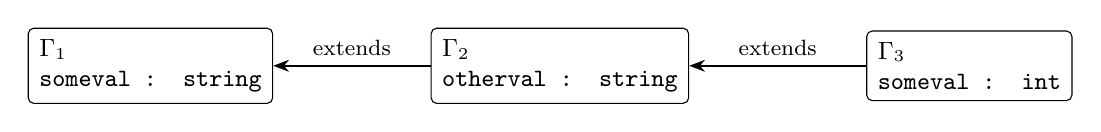
\begin{tikzpicture}[env/.style={draw, rounded corners=2pt, align=left, font=\small, inner sep=4pt}]
  \node[env] (g1) at (0,0) {$\Gamma_1$\\ \texttt{someval : string}};
  \node[env] (g2) at (5.2,0) {$\Gamma_2$\\ \texttt{otherval : string}};
  \node[env] (g3) at (10.4,0) {$\Gamma_3$\\ \texttt{someval : int}};
  \draw[flecha] (g2) -- node[above, font=\footnotesize] {extends} (g1);
  \draw[flecha] (g3) -- node[above, font=\footnotesize] {extends} (g2);
\end{tikzpicture}
\caption{Nested type environments. In $\Gamma_3$, $\Gamma_3 \vdash \mathtt{someval} : \mathit{int}$ because the search stops at the innermost declaration.}
\label{fig:tenv}
\end{figure}

\subsection{Exercises}

\begin{exercise}
What would be the rule for the definition of functions in LETREC? How does the
checker know the type of the parameter?
\end{exercise}

\paragraph{Solution.} It is \textsc{Abs}: if the body has type $T_2$ when the
parameter has type $T_1$, the function has type $T_1 \to T_2$. The parameter's
type is written by the programmer in the typed language
(\texttt{proc (x : int) \dots}); without the annotation it has to be inferred
from how the body uses $x$.

\begin{exercise}
Give the typing derivation of
\texttt{letrec int double (x : int) = if zero?(x) then 0 else -((double -(x,1)), -2) in double}.
\end{exercise}

\paragraph{Solution.} With $\Gamma = \{\mathit{double} : \mathit{int} \to \mathit{int}\}$ and
$\Gamma' = \Gamma, x : \mathit{int}$. In $\Gamma'$: $\mathtt{zero?}(x) : \mathit{bool}$ by
\textsc{Pred} and \textsc{Var}; $0 : \mathit{int}$; $\mathtt{-}(x, 1) : \mathit{int}$ by
\textsc{Diff}; $(\mathit{double}\ \mathtt{-}(x,1)) : \mathit{int}$ by \textsc{Reduc}, since
$\mathit{double} : \mathit{int} \to \mathit{int}$; $\mathtt{-}(\dots, -2) : \mathit{int}$ by
\textsc{Diff}; so the \texttt{if} has type $\mathit{int}$ by \textsc{If}, which matches
the declared result. Then the body \texttt{double} has type $\mathit{int} \to \mathit{int}$
in $\Gamma$ by \textsc{Var}, and by \textsc{Letrec} the whole program has type
$\mathit{int} \to \mathit{int}$.

\begin{exercise}
Which rule fails for \texttt{if zero?(1) then 1 else zero?(0)}?
\end{exercise}

\paragraph{Solution.} \textsc{If}: the condition is a $\mathit{bool}$, but the branches
have types $\mathit{int}$ and $\mathit{bool}$, and the rule requires the same type
$T$ for both. The Rascal checker reports
\texttt{Types did not match \dots: bool != int}.

\begin{exercise}
In the OCaml example, what does \texttt{Printf.printf "\%d \%s" someval otherval}
print if the inner \texttt{let someval = 3} is removed? Does the program still
type check?
\end{exercise}

\paragraph{Solution.} It does not type check: \texttt{someval} is now the outer
one, a \texttt{string}, and \texttt{\%d} requires an \texttt{int}. The format
string makes the types of the arguments part of the check.

% !TeX root = ../main.tex
\section{Lambda calculus}
\label{sec:lambda}

This section and the next go beyond the slides; they give the formal basis
for the rule \textsc{Abs} and for Section~\ref{sec:safety}. The lambda
calculus is a formal system in which everything is a function. A LETREC
\texttt{proc (x) body} is a lambda abstraction $\lambda x.\, \mathit{body}$, and the
application \texttt{(f e)} is the application $f\ e$.

\subsection{Syntax}

There are three constructs: variables $x, y, z, \dots$; abstraction
$\lambda x.\, e$, a function with parameter $x$ and body $e$; and application
$e_1\, e_2$, which applies $e_1$ to $e_2$. Application associates to the left
($f\,a\,b$ is $(f\,a)\,b$), and the body of an abstraction extends as far to
the right as possible. Figure~\ref{fig:lambda-ast} shows the abstract syntax
tree of $(\lambda x.\, x\, x)\,(\lambda y.\, y)$.

\begin{figure}[h]
\centering
\begin{forest}
  for tree={font=\small, s sep=5mm, l sep=4mm},
  [app
    [$\lambda x$ [app [$x$] [$x$]]]
    [$\lambda y$ [$y$]]
  ]
\end{forest}
\caption{Abstract syntax tree of $(\lambda x.\, x\, x)\,(\lambda y.\, y)$.}
\label{fig:lambda-ast}
\end{figure}

\paragraph{Free and bound variables.} In $\lambda x.\, M$ the variable $x$ is
\textbf{bound}: the abstraction is its scope. A variable that is not inside an
abstraction for it is \textbf{free}. In $\lambda x.\, x\, y$, $x$ is bound and
$y$ is free. The name of a bound variable does not matter, as long as renaming
does not capture another variable: $\lambda x.\, x \equiv_\alpha \lambda y.\, y$
($\alpha$-equivalence).

\subsection{Reduction}

Computation is one rule, $\beta$-reduction, which substitutes the argument into
the body:
\[
(\lambda x.\, e)\, v \;\to_\beta\; e[x := v].
\]
A second rule, $\eta$-reduction, says that a function that only passes its
argument on is the function itself: $\lambda x.\, (f\, x) \to_\eta f$ when $x$ is
not free in $f$.

For $(\lambda x.\, x\, x)\,(\lambda y.\, y)$:
\[
(\lambda x.\, x\, x)\,(\lambda y.\, y) \;\to_\beta\; (\lambda y.\, y)\,(\lambda y.\, y)
\;\to_\beta\; \lambda y.\, y.
\]
The result has no more redexes (subterms of the form $(\lambda x.\, e)\, v$); it is
in normal form.

\paragraph{Evaluation strategies.} When a term has several redexes, the order
matters. Normal order reduces the leftmost, outermost redex first, and finds
a normal form whenever one exists. Call by value evaluates the argument before
the call, as C, Java and Python do. Call by name passes the argument
unevaluated, which is the basis of lazy evaluation. The runtime block
returns to these strategies with the lecture's examples.

\subsection{Church encodings}

The pure calculus has no numbers or booleans, but they can be encoded as
functions. A boolean chooses between two alternatives:
\[
\mathit{TRUE} \equiv \lambda t.\, \lambda f.\, t \qquad
\mathit{FALSE} \equiv \lambda t.\, \lambda f.\, f \qquad
\mathit{AND} \equiv \lambda p.\, \lambda q.\, p\, q\, p.
\]
A Church numeral $n$ applies a function $n$ times:
\[
0 \equiv \lambda f.\, \lambda x.\, x \qquad
1 \equiv \lambda f.\, \lambda x.\, f\, x \qquad
2 \equiv \lambda f.\, \lambda x.\, f\,(f\, x) \qquad
\mathit{SUCC} \equiv \lambda n.\, \lambda f.\, \lambda x.\, f\,(n\, f\, x).
\]

\subsection{Recursion}

Abstractions are anonymous, so a function cannot call itself by name. LETREC
solves this with \texttt{letrec}, which puts the function in its own scope.
The pure calculus uses a fixed-point combinator:
\[
Y = \lambda f.\, (\lambda x.\, f\,(x\, x))\,(\lambda x.\, f\,(x\, x)).
\]
One step of reduction shows that $Y\, g \to_\beta (\lambda x.\, g\,(x\, x))\,(\lambda x.\, g\,(x\, x)) \to_\beta g\,((\lambda x.\, g\,(x\, x))\,(\lambda x.\, g\,(x\, x)))$,
and the argument of $g$ is again the term that $Y\, g$ reduced to. So
$Y\, g$ behaves as $g\,(Y\, g)$: it gives $g$ a copy of itself.

\subsection{Exercises}

\begin{exercise}
Define $\mathit{OR}$ and $\mathit{NOT}$ with Church booleans and check that
$\mathit{OR}\ \mathit{TRUE}\ \mathit{FALSE}$ reduces to $\mathit{TRUE}$.
\end{exercise}

\paragraph{Solution.} $\mathit{OR} \equiv \lambda p.\, \lambda q.\, p\, p\, q$ and
$\mathit{NOT} \equiv \lambda p.\, p\, \mathit{FALSE}\, \mathit{TRUE}$. Then
$\mathit{OR}\ \mathit{TRUE}\ \mathit{FALSE} \to_\beta \mathit{TRUE}\ \mathit{TRUE}\ \mathit{FALSE}
\to_\beta \mathit{TRUE}$, because $\mathit{TRUE}$ returns its first argument.

\begin{exercise}
Show that $\mathit{SUCC}\ 1$ reduces to $2$.
\end{exercise}

\paragraph{Solution.} $\mathit{SUCC}\ 1 \to_\beta \lambda f.\, \lambda x.\, f\,(1\, f\, x)$,
and $1\, f\, x = (\lambda f.\, \lambda x.\, f\, x)\, f\, x \to_\beta f\, x$, so the result is
$\lambda f.\, \lambda x.\, f\,(f\, x) = 2$.

\begin{exercise}
Which variables are free in $\lambda x.\, (\lambda y.\, x\, y\, z)\, y$?
\end{exercise}

\paragraph{Solution.} $z$, and the last $y$, which is outside the abstraction
$\lambda y$. The first $y$ and $x$ are bound.

% !TeX root = ../main.tex
\section{Simply typed lambda calculus}
\label{sec:stlc}

The untyped calculus accepts terms such as $\mathit{TRUE}\ 3$ or $x\, x$. The
\textbf{simply typed lambda calculus} (STLC) adds the smallest type discipline:
every term has a type, and an application is legal only when the types
match. Its rules are the rules of LETREC (Section~\ref{sec:letrec}) for
variables, functions, application and \texttt{if}; LETREC adds numbers,
\texttt{let} and recursion.

\subsection{Types and terms}

Types are built from two base types and the function type:
\[
\tau ::= \tyint \mid \tybool \mid \tau \to \tau.
\]
Terms are those of the untyped calculus, with an annotation on each parameter,
plus literals and conditionals:
\[
e ::= x \mid \lambda x{:}\tau.\, e \mid e\, e \mid n \mid \ift{e}{e}{e}.
\]

\subsection{The typing judgment}

\begin{mathpar}
\inferrule*[right=T-Var]{x : \tau \in \Gamma}{\Gamma \vdash x : \tau}
\and
\inferrule*[right=T-Abs]{\Gamma, x : \tau_1 \vdash e : \tau_2}{\Gamma \vdash \lambda x{:}\tau_1.\, e : \tau_1 \to \tau_2}
\and
\inferrule*[right=T-App]{\Gamma \vdash e_1 : \tau_1 \to \tau_2 \\ \Gamma \vdash e_2 : \tau_1}{\Gamma \vdash e_1\, e_2 : \tau_2}
\and
\inferrule*[right=T-If]{\Gamma \vdash e_1 : \tybool \\ \Gamma \vdash e_2 : \tau \\ \Gamma \vdash e_3 : \tau}{\Gamma \vdash \ift{e_1}{e_2}{e_3} : \tau}
\end{mathpar}
The rules are syntax-directed: for each form of term exactly one rule
applies, so checking a term never requires a guess. \textsc{T-App} rejects
$3\, (\lambda x{:}\tyint.\, x)$, because 3 does not have a function type, and
$(\lambda x{:}\tyint.\, x)\ \mathit{true}$, because $\tyint \ne \tybool$.
Figure~\ref{fig:stlc-deriv} shows a derivation.

\begin{figure}[h]
\centering
\begin{mathpar}
\inferrule*[right=T-Abs]
  {\inferrule*[right=T-Abs]
    {\inferrule*[right=T-Var]{x : \tyint \in \{x : \tyint, y : \tybool\}}{x : \tyint, y : \tybool \vdash x : \tyint}}
    {x : \tyint \vdash \lambda y{:}\tybool.\, x : \tybool \to \tyint}}
  {\vdash \lambda x{:}\tyint.\, \lambda y{:}\tybool.\, x : \tyint \to \tybool \to \tyint}
\end{mathpar}
\caption{Typing derivation of $\lambda x{:}\tyint.\, \lambda y{:}\tybool.\, x$.}
\label{fig:stlc-deriv}
\end{figure}

\subsection{Capture-avoiding substitution}

$\beta$-reduction substitutes the argument into the body, $e[x := v]$, and the
substitution must not capture variables. With $e = \lambda y.\, x\, y$ and
$v = y$, replacing $x$ by $y$ textually gives $\lambda y.\, y\, y$, where the $y$
that was free has been captured by $\lambda y$. The fix is to rename the bound
variable first ($\lambda z.\, x\, z$, which is $\alpha$-equivalent) and then
substitute: $\lambda z.\, y\, z$. Compilers often avoid the problem by replacing
names with de Bruijn indices, the distance to the binder.

\subsection{Strong normalization}

\begin{theorem}[Strong normalization]
If $\vdash e : \tau$, every reduction sequence that starts at $e$ ends in a
normal form.
\end{theorem}

So every well-typed STLC program terminates, and STLC is not Turing complete.
The reason is that self-application has no type. For $x\, x$ to be typed, $x$
needs a type $\alpha$ with $\alpha = \alpha \to \beta$, and no finite type satisfies
that equation, because the right side is always bigger than the left. The
combinator $Y$ is built from self-applications, so it has no type either.
Section~\ref{sec:inference} meets the same equation as the occurs check of
\texttt{proc (f) zero?((f f))}, and Section~\ref{sec:recursive} adds recursive
types to give it a solution. LETREC recovers recursion directly with
\texttt{letrec}, and that is why it can loop.

\subsection{Propositions as types}

Read as logical formulas, the types of STLC are propositions of
intuitionistic logic, and the well-typed terms are their proofs
(Table~\ref{tab:curry-howard}). \textsc{T-App} is modus ponens: from a proof of
$P \Rightarrow Q$ and a proof of $P$ it gives a proof of $Q$. \textsc{T-Abs} is
conditional proof: to prove $P \Rightarrow Q$, assume $P$ and derive $Q$.

\begin{table}[h]
\centering
\small
\begin{tabular}{l l}
  \toprule
  Logic & Types \\
  \midrule
  proposition & type \\
  proof of $P$ & term of type $P$ \\
  implication $P \Rightarrow Q$ & function type $P \to Q$ \\
  conjunction $P \wedge Q$ & product type $P \times Q$ \\
  modus ponens & application \\
  \bottomrule
\end{tabular}
\caption{The Curry--Howard correspondence.}
\label{tab:curry-howard}
\end{table}

The term $\lambda x{:}\tau_1.\, \lambda y{:}\tau_2.\, x$ of Figure~\ref{fig:stlc-deriv}
is a proof of $P \Rightarrow (Q \Rightarrow P)$. Proof assistants such as Coq and
Agda are built on this correspondence: checking the type of a program is
checking a proof.

\subsection{Exercises}

\begin{exercise}
Is $\lambda x{:}(\tyint \to \tyint).\, x\, x$ well typed?
\end{exercise}

\paragraph{Solution.} No. \textsc{T-App} on $x\, x$ needs the type of the operator,
$\tyint \to \tyint$, to have as argument type the type of the operand,
$\tyint \to \tyint$. But the argument type is $\tyint$, and $\tyint \ne \tyint \to \tyint$.

\begin{exercise}
Perform $(\lambda y.\, x\, (\lambda x.\, x\, y))[x := y\, z]$.
\end{exercise}

\paragraph{Solution.} The outer $\lambda y$ would capture the $y$ of $y\, z$, so rename it
to $w$: $\lambda w.\, x\, (\lambda x.\, x\, w)$. Inside $\lambda x$ the variable $x$ is
bound, so only the first $x$ is replaced: $\lambda w.\, (y\, z)\, (\lambda x.\, x\, w)$.

\begin{exercise}
Write a term of type $(\tau_1 \to \tau_2) \to (\tau_2 \to \tau_3) \to (\tau_1 \to \tau_3)$.
Which logical rule does it prove?
\end{exercise}

\paragraph{Solution.} $\lambda f{:}\tau_1 \to \tau_2.\, \lambda g{:}\tau_2 \to \tau_3.\, \lambda x{:}\tau_1.\, g\,(f\, x)$,
function composition. It proves that implication is transitive: if
$P \Rightarrow Q$ and $Q \Rightarrow R$, then $P \Rightarrow R$.

% !TeX root = ../main.tex
\section{Type inference}
\label{sec:inference}

Writing the types in a program helps with design and documentation, but it
takes time. In a statically typed language the compiler can deduce the types
from the context in which each entity is used. In LETREC this means making the
annotations optional:
\begin{lstlisting}
Expression ::= letrec Type? Identifier (Identifier : Type?) = Expression in Expression
             | proc (Identifier : Type?) Expression
             | ...
Type       ::= int | boolean
\end{lstlisting}
The Rascal grammar of Section~\ref{sec:letrec} already allows a missing type;
the abstract syntax stores it as \texttt{noType()}.

\subsection{Rules with type variables}

When a type is unknown, the checker gives it a name, a \textbf{type variable}
$t_0, t_1, \dots$, and collects equations between types from the rules:
\begin{mathpar}
\inferrule*[right=(Diff)]{e_1 : \mathit{Int} \\ e_2 : \mathit{Int}}{\mathtt{-}(e_1, e_2) : \mathit{Int}}
\and
\inferrule*[right=(Pred)]{e_1 : \mathit{Int}}{\mathtt{zero?}(e_1) : \mathit{Boolean}}
\and
\inferrule*[right=(If)]{e_1 : \mathit{Boolean} \\ e_2 : T \\ e_3 : T}{(\mathtt{if}\ e_1\ \mathtt{then}\ e_2\ \mathtt{else}\ e_3) : T}
\and
\inferrule*[right=(Abs)]{v : T_{\mathit{var}} \\ \mathit{body} : T_{\mathit{body}}}{\mathtt{proc}(v)\ \mathit{body} : T_{\mathit{var}} \to T_{\mathit{body}}}
\and
\inferrule*[right=(Reduc)]{\mathit{rator} : T_1 \to T_2 \\ \mathit{rand} : T_1}{\mathtt{call}(\mathit{rator}, \mathit{rand}) : T_2}
\end{mathpar}
Every use of a rule produces equations. Solving the equations gives the
types.

\paragraph{Example 1.} The lecture starts with
\begin{lstlisting}
letrec foo (x) = if zero?(x) then 1 else -(x, (foo -(x,1))) in foo
\end{lstlisting}
Let $x : t_x$ and $\mathit{foo} : t_x \to t_r$. $\mathtt{zero?}(x)$ gives $t_x = \mathit{Int}$.
The \texttt{then} branch is $1 : \mathit{Int}$, so the \texttt{if} has type
$\mathit{Int}$ and $t_r = \mathit{Int}$. The \texttt{else} branch is a difference,
which needs $(\mathit{foo}\ \mathtt{-}(x,1)) : \mathit{Int}$, consistent with
$t_r = \mathit{Int}$. So $\mathit{foo} : \mathit{Int} \to \mathit{Int}$.

\paragraph{Example 2.} For
\begin{lstlisting}
proc (f) proc (x) -((f 3), (f x))
\end{lstlisting}
the lecture names every subexpression (Figure~\ref{fig:infer-tree}): $t_0$ for the
whole term, $t_1$ for the inner \texttt{proc}, $t_2$ for the difference, $t_3$
for \texttt{(f 3)}, $t_4$ for \texttt{(f x)}, and $t_f$, $t_x$ for the
parameters. The equations are in Table~\ref{tab:infer-eqs}.

\begin{figure}[h]
\centering
\begin{forest}
  for tree={font=\small, s sep=4mm, l sep=4mm, align=center},
  [{\texttt{proc (f)}\\$t_0$}
    [{\texttt{proc (x)}\\$t_1$}
      [{\texttt{-( , )}\\$t_2$}
        [{\texttt{(f 3)}\\$t_3$} [{\texttt{f}\\$t_f$}] [{\texttt{3}\\$\mathit{Int}$}]]
        [{\texttt{(f x)}\\$t_4$} [{\texttt{f}\\$t_f$}] [{\texttt{x}\\$t_x$}]]
      ]
    ]
  ]
\end{forest}
\caption{Type variables for the subexpressions of \texttt{proc (f) proc (x) -((f 3), (f x))}.}
\label{fig:infer-tree}
\end{figure}

\begin{table}[h]
\centering
\small
\begin{tabular}{l l l}
  \toprule
  Subexpression & Rule & Equation \\
  \midrule
  \texttt{(f 3)}         & Reduc & $t_f = \mathit{Int} \to t_3$ \\
  \texttt{(f x)}         & Reduc & $t_f = t_x \to t_4$ \\
  \texttt{-((f 3),(f x))} & Diff & $t_3 = \mathit{Int}$,\ \ $t_4 = \mathit{Int}$,\ \ $t_2 = \mathit{Int}$ \\
  \texttt{proc (x) \dots}  & Abs  & $t_1 = t_x \to t_2$ \\
  \texttt{proc (f) \dots}  & Abs  & $t_0 = t_f \to t_1$ \\
  \bottomrule
\end{tabular}
\caption{Equations for Example 2.}
\label{tab:infer-eqs}
\end{table}

Solving: $t_f = \mathit{Int} \to \mathit{Int}$; from the second equation
$t_x \to \mathit{Int} = \mathit{Int} \to \mathit{Int}$, so $t_x = \mathit{Int}$; then
$t_1 = \mathit{Int} \to \mathit{Int}$ and
\[
t_0 = (\mathit{Int} \to \mathit{Int}) \to \mathit{Int} \to \mathit{Int}.
\]
The function takes a function from integers to integers and returns a
function from integers to integers. The parentheses around the first
$\mathit{Int} \to \mathit{Int}$ matter: the slide writes
$t_0 = \mathit{Int} \to \mathit{Int} \to \mathit{Int} \to \mathit{Int}$, which, since the
arrow associates to the right, would be a function of three integers.

\paragraph{Example 3.} \texttt{if x then -(x,1) else 0}. The difference needs
$t_x = \mathit{Int}$; the condition of the \texttt{if} needs
$t_x = \mathit{Boolean}$. Together, $\mathit{Boolean} = \mathit{Int}$, which has no
solution: the expression has a type error.

\paragraph{Example 4.} \texttt{proc (f) zero?((f f))}. With $f : t_f$ and
$(f\ f) : t_3$, application gives $t_f = t_f \to t_3$, and \texttt{zero?} gives
$t_3 = \mathit{Int}$, so $t_f = t_f \to \mathit{Int}$. The type of $f$ would be defined
in terms of itself, and no finite type satisfies the equation. The
\textbf{occurs check} detects this: a variable cannot be bound to a type that
contains it.

\subsection{The algorithm}

The lecture divides type inference into five parts:
\begin{enumerate}
  \item substitution: replace a type variable by a known type inside a type
    expression;
  \item the no-occurrence property: a variable that is bound never appears
    in the types of the substitution, which the occurs check preserves;
  \item unification: add the equation $t_1 = t_2$ between two types to a
    substitution;
  \item fresh type variables for the expressions whose type is unknown;
  \item the type of an expression, computed from the rules and the current
    substitution.
\end{enumerate}

\paragraph{Substitution.} Substituting a type $t_1$ for a variable $t_{\mathit{var}}$
in a type expression $t_0$ replaces every occurrence:
\[
(t_{\mathit{var}} \to t_x \to t_y \to \mathit{Int} \to t_{\mathit{var}})[t_{\mathit{var}} = T]
\;=\; T \to t_x \to t_y \to \mathit{Int} \to T.
\]
The function goes by cases on $t_0$:
\begin{lstlisting}
substitution(t0, tvar, t1) : Type {
  switch (t0) {
    case int-type(): int-type;
    case boolean-type(): boolean-type;
    case proc-type(arg-type, result-type):
      proc-type(substitution(arg-type, tvar, t1), substitution(result-type, tvar, t1));
    case tvar-type(sn): if (t0 == tvar) then t1 else t0;
  }
}
\end{lstlisting}
(The slide compares \texttt{t1 = tvar} in the last case. The comparison is
between the variable found, $t_0$, and the variable being replaced.) A
substitution maps several variables to types. In Rascal, \texttt{apply} follows
chains such as $t_1 = t_2$, $t_2 = \mathit{Int}$:
\coderange{Rascal}{rascal/src/Infer.rsc}{subst}

\paragraph{Unification.} Given two types, the unifier returns a substitution in
which they are equal:
\begin{enumerate}
  \item apply the current substitution to $t_1$ and $t_2$;
  \item if the results are the same, return the substitution unchanged;
  \item if $t_1$ is a variable, propose $t_1 = t_2$, after the occurs check;
  \item if $t_2$ is a variable, do the same;
  \item if both are function types, unify the argument types and then the
    result types; otherwise ($\mathit{Int}$ against $\mathit{Boolean}$, or a basic
    type against a function type) there is no solution.
\end{enumerate}
\begin{lstlisting}
unifier(t1, t2, subs, exp) : Substitution {
  t1 = apply-substitution(t1, subs);
  t2 = apply-substitution(t2, subs);
  condition (t1 == t2) { subs; }
  tvar-type?(t1) {
    if (no-occurrence?(t1, t2)) extend-substitution(subs, t1, t2);
    else Error(No occurrence violation t1 t2 exp);
  }
  tvar-type?(t2) { ... }
  proc-type?(t1) && proc-type?(t2) {
    subs = unifier(proc-type.arg(t1), proc-type.arg(t2), subs, exp);
    subs = unifier(proc-type.res(t1), proc-type.res(t2), subs, exp);
  }
  else { Error(Unification failure t1 t2 exp); }
}

no-occurrence?(tvar, t) : Boolean {
  switch (t) {
    int-type: true;
    bool-type: true;
    proc-type(args, res): no-occurrence?(tvar, args) && no-occurrence?(tvar, res);
    var-type: not(tvar == t)
  }
}
\end{lstlisting}
In Rascal:
\coderange{Rascal}{rascal/src/Infer.rsc}{unify}

\paragraph{Types for expressions.} A missing annotation becomes a fresh
variable (\texttt{optionaltype-2-type}), and the inference function follows
the rules, calling the unifier at each premise that requires two types to be
equal. For an application it creates a variable for the result and unifies
the type of the operator with $t_{\mathit{rand}} \to t_{\mathit{res}}$:
\coderange{Rascal}{rascal/src/Infer.rsc}{infer}
The tests run the four examples of this section: \texttt{foo} gets
\texttt{int -> int}, Example 2 gets \texttt{(int -> int) -> int -> int}, Example 3
fails with a unification failure and Example 4 with a no-occurrence violation.

\subsection{Principal types and Algorithm W}

This subsection goes beyond the slides. The method above is a version of
Algorithm W, the inference algorithm of ML and Haskell (the Hindley--Milner
type system). Unification, when it succeeds, finds the \textbf{most general
unifier}: every other solution is an instance of it. So every typable term
has a \textbf{principal type}, of which all its other types are instances.
The principal type of \texttt{proc (x) x} is $t_0 \to t_0$; $\mathit{Int} \to \mathit{Int}$
is a valid type for it, but an instance. The Rascal test \texttt{identity}
shows the variable left in the result. Section~\ref{sec:polymorphism} uses this
to give \texttt{let}-bound functions polymorphic types.

Checking and inference are different problems. Checking verifies a type that
is given; inference has to find one. For richer type systems inference can
be undecidable, and many modern languages (Rust, Swift, TypeScript) use
\textbf{bidirectional} checking: some constructs synthesize their type
bottom-up (variables, literals, applications), and others are checked against
a type that comes from the context (an unannotated function passed where a
function type is expected). They need more annotations than ML, and combine
better with subtyping.

\paragraph{Generics in Java.} Java infers the type parameters at each call of a
generic method, a restricted form of the same problem:
\coderange{Java}{java/Generics.java}{generics}
\coderange{Java}{java/Generics.java}{use}
For \texttt{p} the compiler infers \texttt{MyPair<Integer, String>}, for
\texttt{q} and \texttt{result} \texttt{Integer}, and for \texttt{pairs}
\texttt{List<MyPair<Integer, String>>}.

\paragraph{References.} The same method extends to the commands of the
semantics block. A cell has type $\tref{T}$, and commands have type $\unit$:
\begin{mathpar}
\inferrule*[right=T-Deref]{\Gamma \vdash l : \tref{T}}{\Gamma \vdash \deref{l} : T}
\and
\inferrule*[right=T-Assign]{\Gamma \vdash l : \tref{T} \\ \Gamma \vdash e : T}{\Gamma \vdash \assign{l}{e} : \unit}
\and
\inferrule*[right=T-While]{\Gamma \vdash B : \tybool \\ \Gamma \vdash C : \unit}{\Gamma \vdash \whiledo{B}{C} : \unit}
\end{mathpar}
In the program
\[
\begin{array}{l}
\assign{a}{1}\ ;\ \assign{b}{1}\ ;\ \whiledo{\deref{n} < 5}{C} \\
C = \ift{\deref{\mathit{term}} \le 2}{\assign{\mathit{res}}{\deref{n}}}{(\assign{c}{\deref{a} + \deref{b}}\ ;\ \assign{\mathit{res}}{\deref{n}}\ ;\ \assign{a}{\deref{b}}\ ;\ \assign{b}{\deref{c}})}\ ;\ \assign{n}{\deref{n} + 1}
\end{array}
\]
every cell is dereferenced and compared with or added to an integer, so
$n, \mathit{res}, a, b, c, \mathit{term} : \tref{\tyint}$; the conditions are $\tybool$; and
every command, the \texttt{while} included, is $\unit$.

\subsection{Exercises}

\begin{exercise}
What is the inferred type of \texttt{if x then -(x,1) else 0}?
\end{exercise}

\paragraph{Solution.} None. The difference requires $t_x = \mathit{Int}$ and the
condition requires $t_x = \mathit{Boolean}$; unifying $\mathit{Int}$ with
$\mathit{Boolean}$ fails.

\begin{exercise}
Infer the type of \texttt{proc (f) proc (x) (f (f x))}.
\end{exercise}

\paragraph{Solution.} $(f\ x)$ gives $t_f = t_x \to t_1$ and $(f\ (f\ x))$ gives
$t_f = t_1 \to t_2$. Unifying the two function types: $t_x = t_1$ and $t_1 = t_2$.
So $t_f = t_x \to t_x$ and the type is $(t_x \to t_x) \to t_x \to t_x$: apply a function
twice, for any type.

\begin{exercise}
Infer the principal type of $\lambda x.\, \lambda y.\, \lambda z.\, x\, z\, (y\, z)$ (the S
combinator).
\end{exercise}

\paragraph{Solution.} Let $z : \gamma$. $y\, z$ gives $y : \gamma \to \beta$. $x\, z\, (y\, z)$
gives $x : \gamma \to \beta \to \alpha$. The type is
$(\gamma \to \beta \to \alpha) \to (\gamma \to \beta) \to \gamma \to \alpha$.

\begin{exercise}
Run the unifier by hand on $t_f = t_f \to \mathit{Int}$ and say at which step it stops.
\end{exercise}

\paragraph{Solution.} After applying the (empty) substitution the two types are
different, and $t_f$ is a variable, so the unifier proposes
$t_f = t_f \to \mathit{Int}$. The occurs check finds $t_f$ inside $t_f \to \mathit{Int}$ and
reports a no-occurrence violation. Without the check, the substitution would
replace $t_f$ forever.

\section{Polymorphism}
\label{sec:polymorphism}

This section goes beyond the slides. In STLC and in typed LETREC, the identity
function has to be written once per type: \texttt{proc (x : int) x} and
\texttt{proc (x : bool) x} are different programs. Section~\ref{sec:inference}
showed that inference gives \texttt{proc (x) x} the type $t_0 \to t_0$, with a
variable left over. \textbf{Polymorphism} is the name for the features that let
one piece of code work at many types. There are three classical kinds:
\begin{itemize}
  \item parametric: one implementation that behaves the same at every type;
  \item ad hoc: one name with a different implementation per type
    (overloading, type classes);
  \item subtype: one implementation usable at every subtype of the type it
    expects (Section~\ref{sec:subtyping}).
\end{itemize}

\subsection{Parametric polymorphism}

System F abstracts over types the same way $\lambda$ abstracts over values. It
adds the type $\forall \alpha.\, \tau$, type abstraction $\Lambda \alpha.\, e$ and type
application $e\,[\tau]$:
\[
\mathit{id} = \Lambda \alpha.\, \lambda x{:}\alpha.\, x \;:\; \forall \alpha.\, \alpha \to \alpha.
\]
$\mathit{id}\,[\tyint]\ 3$ reduces to $3$ and $\mathit{id}\,[\tybool]\ \mathit{true}$ to
$\mathit{true}$: one term, instantiated twice (Figure~\ref{fig:instances}).
Hindley--Milner, the system behind ML and Haskell, is the fragment of System F
where $\forall$ only appears at the outside of a type and instantiation is
implicit. That restriction is what makes the inference of
Section~\ref{sec:inference} possible.

\begin{figure}[h]
\centering
\begin{forest}
  for tree={font=\small, s sep=10mm, l sep=8mm, edge={->}},
  [$\forall \alpha.\, \alpha \to \alpha$
    [$\tyint \to \tyint$, edge label={node[midway, left, font=\footnotesize]{$\alpha := \tyint$}}]
    [$\tybool \to \tybool$, edge label={node[midway, right, font=\footnotesize]{$\alpha := \tybool$}}]
  ]
\end{forest}
\caption{A polymorphic type and two of its instances.}
\label{fig:instances}
\end{figure}

\paragraph{Generalization happens at \texttt{let}.} In Haskell
\codelines{Haskell}{haskell/Polymorphism.hs}{3}{5}
type checks: the \texttt{let}-bound \texttt{ident} gets the type
$\forall \alpha.\, \alpha \to \alpha$, and each use instantiates it. The same thing with a
parameter, \lstinline|(\i -> (i 3, i True)) (\x -> x)|, is rejected with
\texttt{No instance for 'Num Bool'}: a parameter has one type in its whole
body, so after \lstinline|i 3| fixes it to a function on numbers, \lstinline|i True|
fails. Algorithm W quantifies the free type variables of a \texttt{let}-bound
value (they cannot appear in the context), and never those of a parameter.
ML restricts generalization further to values (the value restriction): a
generalized mutable cell could store a value at one type and be read at
another.

\subsection{Ad hoc polymorphism}

Overloading binds one name to unrelated implementations, chosen at compile
time by the types of the arguments:
\codelines{Java}{java/Overloading.java}{2}{3}
Haskell's type classes give this a structure: a class declares operations
and each instance implements them for one type. A function constrained by a
class is parametric in the type and ad hoc in the operation it calls:
\codelines{Haskell}{haskell/Polymorphism.hs}{7}{19}
Java gets the same effect with an interface as a bound on a type parameter
(Rust uses traits for this):
\codelines{Java}{java/Overloading.java}{5}{12}

\subsection{Higher-rank polymorphism}

Hindley--Milner only allows $\forall$ at the outside of a type. A function that
receives a polymorphic function and uses it at two types needs a $\forall$
inside the argument, a rank-2 type:
\codelines{Haskell}{haskell/Polymorphism.hs}{21}{22}
Inference cannot find this type (the first use would fix the type of
\texttt{f}), but checking against the written signature works. Haskell allows
it with the \texttt{RankNTypes} extension.

\subsection{Exercises}

\begin{exercise}
Write the System F term and type of \textit{const}, with
$\mathit{const}\ x\ y = x$. What is the normal form of
$\mathit{const}\,[\tyint]\,[\tybool]\ 3\ \mathit{true}$?
\end{exercise}

\paragraph{Solution.} $\Lambda \alpha.\, \Lambda \beta.\, \lambda x{:}\alpha.\, \lambda y{:}\beta.\, x : \forall \alpha.\, \forall \beta.\, \alpha \to \beta \to \alpha$.
The application reduces to $3$.

\begin{exercise}
What does the inference of Section~\ref{sec:inference} say about
\texttt{let i = proc (x) x in if (i zero?(0)) then (i 1) else 2}? Would the
program type check with let-polymorphism?
\end{exercise}

\paragraph{Solution.} It fails. The inference of Section~\ref{sec:inference} does
not generalize, so \texttt{i} has one type $t \to t$ in the whole body.
\texttt{(i zero?(0))} gives $t = \mathit{Boolean}$ and \texttt{(i 1)} gives
$t = \mathit{Int}$, and unification fails. With let-polymorphism \texttt{i} would get
$\forall t.\, t \to t$, each use would have its own instance, and the program
would have type $\mathit{Int}$.

\section{Subtyping}
\label{sec:subtyping}

This section goes beyond the slides, except for the example of variance,
which comes from the statement of the course project. \textbf{Subtyping} asks
when a term of one type can be used where another type is expected. The
answer is a relation $\tau_1 <: \tau_2$, read ``$\tau_1$ is a subtype of
$\tau_2$'': anywhere a $\tau_2$ is expected, a $\tau_1$ will do.

\subsection{Subsumption}

Subtyping enters the type system through one rule:
\begin{mathpar}
\inferrule*[right=T-Sub]{\Gamma \vdash e : \tau_1 \\ \tau_1 <: \tau_2}{\Gamma \vdash e : \tau_2}
\end{mathpar}
The other rules do not change; the design work is in the definition of $<:$.

\paragraph{Records.} A record with more fields is a subtype of a record with
fewer, if the shared fields agree (width subtyping):
$\{\mathit{name}: \mathit{string}, \mathit{age}: \tyint, \mathit{email}: \mathit{string}\} <:
\{\mathit{name}: \mathit{string}, \mathit{age}: \tyint\}$. A function that only reads
\texttt{name} and \texttt{age} can ignore \texttt{email}. A record is also a
subtype if each field is a subtype of the corresponding field (depth
subtyping).

\subsection{Variance}

How does subtyping extend to type constructors? For functions the rule is
\begin{mathpar}
\inferrule*[right=S-Arrow]{\sigma_1 <: \tau_1 \\ \tau_2 <: \sigma_2}{\tau_1 \to \tau_2 \;<:\; \sigma_1 \to \sigma_2}
\end{mathpar}
The argument goes in the opposite direction. A caller that expects
$\sigma_1 \to \sigma_2$ will pass any $\sigma_1$, so the function must accept at least
that: $\sigma_1 <: \tau_1$. The caller will use the result as a $\sigma_2$, so the
function may return something more specific: $\tau_2 <: \sigma_2$. Function types
are \textbf{contravariant} in the argument and \textbf{covariant} in the result.

The statement of the course project (Objectilang) has an example. With
\texttt{Puppy <: Dog <: Animal} and \texttt{DogFood <: Food}, a generic
\texttt{Transformer[-In, +Out]} declares \texttt{In} contravariant and
\texttt{Out} covariant, so
\[
\mathtt{Transformer[Animal, DogFood]} \;<:\; \mathtt{Transformer[Puppy, Food]}.
\]
A transformer that accepts any animal and returns dog food can be used where
the program needs one that accepts puppies and returns some food
(Figure~\ref{fig:variance}). The comments of the statement say the same thing:
the input is broader and the output narrower.

\begin{figure}[h]
\centering
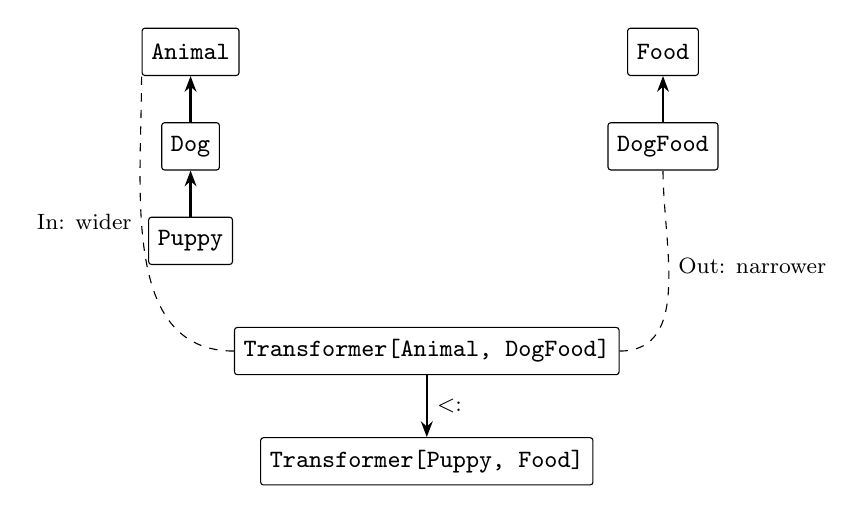
\begin{tikzpicture}[box/.style={draw, rounded corners=1pt, font=\small\ttfamily, minimum height=6mm}]
  \node[box] (animal) at (0,2.4) {Animal};
  \node[box] (dog) at (0,1.2) {Dog};
  \node[box] (puppy) at (0,0) {Puppy};
  \node[box] (food) at (6,2.4) {Food};
  \node[box] (dogfood) at (6,1.2) {DogFood};
  \draw[flecha] (dog) -- (animal);
  \draw[flecha] (puppy) -- (dog);
  \draw[flecha] (dogfood) -- (food);
  \node[box] (t1) at (3,-1.4) {Transformer[Animal, DogFood]};
  \node[box] (t2) at (3,-2.8) {Transformer[Puppy, Food]};
  \draw[flecha] (t1) -- node[right, font=\footnotesize] {$<:$} (t2);
  \draw[dashed] (t1.west) to[out=180, in=270] node[left, font=\footnotesize, pos=0.6] {In: wider} (animal.south west);
  \draw[dashed] (t1.east) to[out=0, in=270] node[right, font=\footnotesize, pos=0.6] {Out: narrower} (dogfood.south);
\end{tikzpicture}
\caption{Subtype hierarchies (arrows point to the supertype) and the variance of \texttt{Transformer[-In, +Out]}.}
\label{fig:variance}
\end{figure}

Java expresses variance at the use of a generic type, with wildcards:
\codelines{Java}{java/Flyer.java}{8}{11}
\texttt{List<? extends Animal>} accepts a \texttt{List<Dog>}: reading animals
from it is safe. Writing is not, which is why a mutable list cannot be
covariant without the wildcard.

\paragraph{Liskov substitution.} In object-oriented design the same idea is the
Liskov substitution principle: if $S$ is a subtype of $T$, objects of type $T$
can be replaced by objects of type $S$ without breaking the program.
Subsumption is the typing side of it; the variance rules keep it sound.

\subsection{Nominal and structural subtyping}

In a \textbf{nominal} system the relation has to be declared. In Java a class
is a subtype of an interface only if it says \texttt{implements}:
\codelines{Java}{java/Flyer.java}{2}{6}
Without \texttt{implements Flying}, \texttt{Flying f = new Duck();} is rejected
with \texttt{incompatible types: Duck cannot be converted to Flying}, even
though \texttt{Duck} has the method. In a \textbf{structural} system the shape is
enough: in TypeScript and in Go, a value with a method \texttt{fly} satisfies an
interface that requires it, without mentioning the interface. Duck typing
(Section~\ref{sec:types}) is the dynamic version of structural typing.

\subsection{Exercises}

\begin{exercise}
Is $\mathit{Animal} \to \mathit{Dog}$ a subtype of $\mathit{Dog} \to \mathit{Animal}$? And the
other way around?
\end{exercise}

\paragraph{Solution.} By S-Arrow, $\mathit{Animal} \to \mathit{Dog} <: \mathit{Dog} \to \mathit{Animal}$
needs $\mathit{Dog} <: \mathit{Animal}$ (argument) and $\mathit{Dog} <: \mathit{Animal}$ (result).
Both hold, so yes. The other way around needs $\mathit{Animal} <: \mathit{Dog}$, which
does not hold.

\begin{exercise}
With \texttt{Transformer[-In, +Out]}, which of these relations hold?
\begin{enumerate}
  \item \texttt{Transformer[Dog, Food]} $<:$ \texttt{Transformer[Animal, Food]}
  \item \texttt{Transformer[Animal, DogFood]} $<:$ \texttt{Transformer[Dog, DogFood]}
\end{enumerate}
\end{exercise}

\paragraph{Solution.} The first does not hold: \texttt{In} is contravariant, so
the input on the right (\texttt{Animal}) would have to be a subtype of the
input on the left (\texttt{Dog}). A caller that expects to pass any animal
could pass a cat. The second holds: \texttt{Dog <: Animal} for the input, and
the output is the same.

% !TeX root = ../main.tex
\section{Recursive types}
\label{sec:recursive}

The inductive types of Section~\ref{sec:types} are defined by constants and
constructors that refer to the type being defined: $0 : \mathbb{N}$ and
$s : \mathbb{N} \to \mathbb{N}$. This section, which goes beyond the slides, shows how a
type system expresses that self-reference. A list of integers is either empty
or an integer followed by another list:
\[
\alpha = \unit + (\tyint \times \alpha).
\]
With the types of STLC this equation has no solution. Expanding it never ends,
$\alpha = \unit + \tyint \times (\unit + \tyint \times (\dots))$, for the same reason that
$t_f = t_f \to \mathit{Int}$ failed the occurs check in Section~\ref{sec:inference}.

\subsection{$\mu$-types}

A new type former names the solution: $\mu\alpha.\, \tau$ is the type $\alpha$ that
satisfies $\alpha = \tau$, where $\tau$ may mention $\alpha$.
\[
\mathbf{List}\ \tyint = \mu\alpha.\, \unit + (\tyint \times \alpha)
\qquad
\mathbf{Tree} = \mu\alpha.\, \tyint + (\alpha \times \tyint \times \alpha)
\qquad
\mathbb{N} = \mu\alpha.\, \unit + \alpha
\]
In the last one, $\unit$ plays the role of $0$ and the right side of the sum
the role of $s$.

\paragraph{Fold and unfold.} The values of $\mu\alpha.\, \tau$ are related to its
unfolding $\tau[\mu\alpha.\tau / \alpha]$ (the body with the whole type put back for
$\alpha$) by two operations:
\begin{mathpar}
\inferrule*[right=T-Fold]{\Gamma \vdash e : \tau[\mu\alpha.\tau / \alpha]}{\Gamma \vdash \mathbf{fold}(e) : \mu\alpha.\, \tau}
\and
\inferrule*[right=T-Unfold]{\Gamma \vdash e : \mu\alpha.\, \tau}{\Gamma \vdash \mathbf{unfold}(e) : \tau[\mu\alpha.\tau / \alpha]}
\end{mathpar}
$\mathbf{fold}$ packages one layer (what a constructor such as \textit{cons}
does) and $\mathbf{unfold}$ opens one layer (what a pattern match does).
Figure~\ref{fig:folds} shows the list $[1, 2]$ built with three folds, one per
constructor.

\begin{figure}[h]
\centering
\begin{forest}
  for tree={font=\small, s sep=4mm, l sep=4mm},
  [fold
    [{$\mathit{inr}$}
      [$\times$ [1]
        [fold
          [{$\mathit{inr}$}
            [$\times$ [2] [fold [{$\mathit{inl}$} [$()$]]]]
          ]
        ]
      ]
    ]
  ]
\end{forest}
\caption{The list $[1, 2]$ as a value of $\mu\alpha.\, \unit + (\tyint \times \alpha)$. $\mathit{inl}$ and $\mathit{inr}$ choose a side of the sum.}
\label{fig:folds}
\end{figure}

Languages with explicit fold and unfold, and a type equality that only
compares syntax, are \emph{iso-recursive}; languages where $\mu\alpha.\, \tau$ and its
unfolding are the same type are \emph{equi-recursive}, and need a more complex
equality on infinite trees. ML-family languages are iso-recursive, which fits
their inference.

\subsection{Algebraic data types}

The data types of Haskell are recursive types where the constructors are the
folds and pattern matching is the unfold:
\coderange{Haskell}{haskell/RecursiveTypes.hs}{types}
\coderange{Haskell}{haskell/RecursiveTypes.hs}{functions}
\texttt{Cons} takes an element and a list (one unfolding of the type) and
returns a list; the equation \texttt{len (Cons \_ xs)} opens one layer.
Recursive types do not reopen what the occurs check closed: ordinary type
variables still cannot refer to themselves, and self-reference is allowed
only where a $\mu$ (a \texttt{data} declaration) introduces it.

\subsection{Exercises}

\begin{exercise}
Unfold $\mathbf{List}\ \tyint$ one level.
\end{exercise}

\paragraph{Solution.} $\unit + (\tyint \times \mu\alpha.\, \unit + (\tyint \times \alpha))$, that is,
$\unit + (\tyint \times \mathbf{List}\ \tyint)$: empty, or an integer and a list.

\begin{exercise}
Give a $\mu$-type for nonempty lists of booleans.
\end{exercise}

\paragraph{Solution.} $\mu\alpha.\, \tybool + (\tybool \times \alpha)$: the base case is a single
boolean instead of $\unit$.

\begin{exercise}
Why does Rust reject \texttt{enum List<T> \{ Nil, Cons(T, List<T>) \}} and
accept \texttt{Cons(T, Box<List<T>>)}?
\end{exercise}

\paragraph{Solution.} Rust stores the fields of an \texttt{enum} inline, so a
\texttt{List} would contain a \texttt{List} and have infinite size.
\texttt{Box} stores a pointer, of fixed size, to a list on the heap. Haskell
and ML represent recursive values with pointers by default, which is why
they need no annotation.

% !TeX root = ../main.tex
\section{Type safety}
\label{sec:safety}

This section goes beyond the slides. Type safety is the formal version of
``well-typed programs cannot go wrong'': a well-typed program never reaches a
state where no rule applies. It is proved as two theorems.

\begin{theorem}[Progress]
If $\vdash e : \tau$, then $e$ is a value or there is an $e'$ with $e \reduces e'$.
\end{theorem}

\begin{theorem}[Preservation]
If $\vdash e : \tau$ and $e \reduces e'$, then $\vdash e' : \tau$.
\end{theorem}

Together they give safety: start from a well-typed term; progress says it is a
value or it can take a step, and preservation says that after the step it is
still well typed with the same type, so progress applies again
(Figure~\ref{fig:safety}). The evaluation either ends in a value of type
$\tau$ or runs forever, as in the \texttt{letrec} loop of
Section~\ref{sec:types}; it never gets stuck.

\begin{figure}[h]
\centering
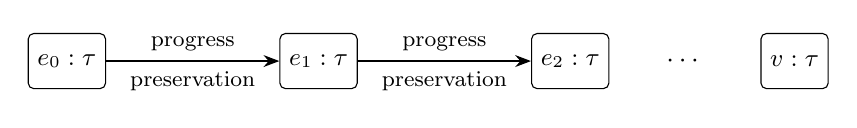
\begin{tikzpicture}[node distance=2.2cm, box/.style={draw, rounded corners=2pt, font=\small, minimum height=7mm}]
  \node[box] (e0) {$e_0 : \tau$};
  \node[box, right=of e0] (e1) {$e_1 : \tau$};
  \node[box, right=of e1] (e2) {$e_2 : \tau$};
  \node[right=0.6cm of e2] (dots) {$\cdots$};
  \node[box, right=0.6cm of dots] (v) {$v : \tau$};
  \draw[flecha] (e0) -- node[above, font=\footnotesize] {progress} node[below, font=\footnotesize] {preservation} (e1);
  \draw[flecha] (e1) -- node[above, font=\footnotesize] {progress} node[below, font=\footnotesize] {preservation} (e2);
\end{tikzpicture}
\caption{Each step exists by progress and keeps the type by preservation.}
\label{fig:safety}
\end{figure}

\subsection{Lemmas}

\begin{lemma}[Canonical forms]
If $v$ is a value and $\vdash v : \tau$, the form of $v$ is determined by $\tau$:
if $\tau = \tybool$ then $v$ is $\mathit{true}$ or $\mathit{false}$; if $\tau = \tau_1 \to \tau_2$
then $v = \lambda x{:}\tau_1.\, e$.
\end{lemma}

\begin{lemma}[Substitution]
If $\Gamma, x : \tau' \vdash e : \tau$ and $\Gamma \vdash v : \tau'$, then
$\Gamma \vdash e[x := v] : \tau$.
\end{lemma}

Canonical forms lets a proof split cases on the form of a value; substitution
handles the $\beta$-reduction case of preservation: the body $e$ was typed
assuming $x : \tau'$, and the argument has type $\tau'$.

\subsection{Proof strategy}

Both theorems are proved by induction on the typing derivation, with one case
per rule. For progress with \textsc{T-App}, $e = e_1\, e_2$: by the induction
hypothesis $e_1$ is a value or takes a step. If it takes a step, so does
$e_1\, e_2$. If it is a value, its type is a function type, so by canonical
forms it is a $\lambda$; then the same reasoning applies to $e_2$, and when both are
values $e_1\, e_2$ is a $\beta$-redex and takes a step. The rules of LETREC
(Section~\ref{sec:letrec}) are the cases a proof for LETREC would cover; the
case \textsc{Diff}, for example, uses canonical forms to know that both
operands of a difference are numbers when they are values.

\subsection{Exercises}

\begin{exercise}
Prove progress for \textsc{T-If}, assuming it for the condition.
\end{exercise}

\paragraph{Solution.} Let $e = \ift{e_1}{e_2}{e_3}$ with $\vdash e_1 : \tybool$. By the
induction hypothesis $e_1$ is a value or takes a step. If it takes a step,
$e$ steps by reducing the condition. If it is a value, by canonical forms it
is $\mathit{true}$ or $\mathit{false}$, and $e$ steps to $e_2$ or $e_3$.

\begin{exercise}
Give a term that is stuck and show which typing rule rejects it.
\end{exercise}

\paragraph{Solution.} $3\ 4$ (in LETREC, \texttt{(3 4)}) is not a value and no rule
reduces it. \textsc{T-App} (\textsc{Reduc}) requires the operator to have a
function type, and $3 : \tyint$, so the term is not well typed. The Rascal test
\texttt{notProc} of \texttt{Letrec.rsc} checks this.


\bibliographystyle{plain}
\bibliography{../../common/bibliography,references}

\end{document}
